\subsection{Requerimientos del usuario.}

En esta sección se describen los requerimientos del usuario, los cuales representan las expectativas y servicios que esperan los usuarios finales de la aplicación web. Estos requerimientos han sido identificados con base al análisis del problema, con el objetivo de propiciar que la solución desarrollada sea útil.

Los requerimientos del usuario se definen, de manera general, qué debe hacer la aplicación web desde la perspectiva del usuario en un lenguaje natural, sin entregar detalles técnicos de implementación. Estos servirán como base para la definición de requerimientos funcionales y no funcionales. 

\begin{tabularx}{\textwidth}{|>{\centering\arraybackslash}m{2cm}|m{3.6cm}|Y|>{\centering\arraybackslash}m{2.0cm}|}
\caption{Requerimientos del usuario.}
\label{tab:ru} \\

\hline
\textbf{ID} & \textbf{Nombre} & \textbf{Descripción} & \textbf{Prioridad} \\
\hline
\endfirsthead

\hline
\textbf{ID} & \textbf{Nombre} & \textbf{Descripción} & \textbf{Prioridad} \\
\hline
\endhead

\hline
\endfoot

% RU-01
RU-01 &
Registro de usuarios. &
La aplicación web debe permitir el registro de usuarios. El tutor se registra de forma autónoma, mientras que los alumnos son registrados por el tutor, asociándolos a su grado y grupo. &
Alta \\
\hline

% RU-02
RU-02 &
Autenticación de usuario. &
El usuario debe poder autenticarse en la aplicación web para acceder a sus funcionalidades de acuerdo con su rol. &
Alta \\
\hline

% RU-03
RU-03 &
Visualización de estado de alumnos. &
El tutor debe poder visualizar el estado de desempeño de sus alumnos, clasificándolos como bajo desempeño, desempeño regular y desempeño de excelencia, con el fin de identificar su progreso. &
Alta \\
\hline

% RU-04
RU-04 &
Clasificación de alumnos. &
La aplicación web debe mostrar un gráfico con la cantidad de alumnos clasificados según su nivel de desempeño (bajo, regular y excelencia), actualizándose conforme a los resultados obtenidos en ortografía y legibilidad. &
Media \\
\hline

% RU-05
RU-05 &
Visualización de ejercicios. &
La aplicación web debe permitir observar los ejercicios disponibles. &
Alta \\
\hline

% RU-06
RU-06 &
Activación de ejercicios. &
El tutor debe poder activar ejercicios a su elección, estableciendo una fecha límite de entrega cuando lo considere necesario. &
Alta \\
\hline

% RU-07
RU-07 &
Visualización de ejercicios seleccionados. &
La aplicación web debe mostrar los ejercicios seleccionados por el tutor y su fecha límite de entrega. &
Media \\
\hline

% RU-08
RU-08 &
Visualización de ejercicios pendientes. &
El alumno debe poder observar los ejercicios asignados y su fecha límite de entrega, para una correcta organización y cumplimiento de sus actividades en tiempo. &
Alta \\
\hline

% RU-09
RU-09 &
Visualización de ejercicios vencidos por tutor. &
La aplicación web debe permitir al tutor consultar los ejercicios cuya fecha límite ha expirado, para poder extender el plazo de entrega si lo considera necesario. &
Media \\
\hline

% RU-10
RU-10 &
Visualización de ejercicios vencidos por alumno. &
El alumno debe poder observar los ejercicios que no completó a tiempo, para conocer su estado y saber si el tutor ya habilitó su entrega. &
Media \\
\hline

% RU-11
RU-11 &
Realizar intento de ejercicios pendientes. &
El alumno debe poder realizar el ejercicio seleccionado por el tutor en una vista de captura de escritura. &
Alta \\
\hline

% RU-12
RU-12 &
Escritura digital en lienzo. &
El alumno debe poder escribir directamente sobre un lienzo digital, contando con herramientas de goma y deshacer para corregir su trazo, con el fin de realizar el ejercicio de escritura manuscrita desde el dispositivo. &
Alta \\
\hline

% RU-13
RU-13 &
Carga de fotografía como alternativa. &
El alumno debe poder subir una fotografía de su escritura manuscrita en papel como alternativa al lienzo digital, para adaptarse a distintas condiciones de acceso. &
Alta \\
\hline

% RU-14
RU-14 &
Envío del ejercicio para revisión. &
El alumno debe poder enviar su ejercicio a la aplicación web para que sea analizado, una vez que considere que su escritura está lista. &
Alta \\
\hline

% RU-15
RU-15 &
Visualización de ejercicios completados. &
El alumno debe poder observar los ejercicios completados, así como sus resultados de escritura. &
Media \\
\hline

% RU-16
RU-16 &
Visualización de ejercicios completados por alumno. &
La aplicación web debe permitir al tutor observar las actividades realizadas por cada alumno, incluyendo sus resultados. &
Media \\
\hline

% RU-17
RU-17 &
Modificación de resultados. &
El tutor debe poder modificar los resultados de un ejercicio realizado por el alumno, en caso de no estar de acuerdo con el análisis ortográfico y caligráfico. &
Baja \\
\hline

% RU-18
RU-18 &
Visualización de actividades sugeridas. &
El alumno debe poder observar las actividades sugeridas por la aplicación web, correspondientes a sus análisis ortográficos y caligráficos. &
Media \\
\hline

% RU-19
RU-19 &
Realizar actividades sugeridas. &
El alumno debe poder realizar las actividades sugeridas por la aplicación web, para trabajar en la mejora de los aspectos detectados en su escritura. &
Media \\
\hline

\end{tabularx}

%------- Reglas de negocio

\subsection{Reglas de negocio}

\begin{tabularx}{\textwidth}{|>{\centering\arraybackslash}m{2cm}|m{3.6cm}|Y|>{\centering\arraybackslash}m{2.0cm}|}
\caption{Reglas de negocio.}
\label{tab:rn} \\

\hline
\textbf{ID} & \textbf{Nombre} & \textbf{Descripción}  \\
\hline
\endfirsthead

\hline
\textbf{ID} & \textbf{Nombre} & \textbf{Descripción}  \\
\hline
\endhead

\hline
\endfoot

RN-01 & Registro de tutores &
Todo usuario que actúe como tutor debe estar registrado en el sistema con el rol de tutor. \\ \hline

RN-02 & Registro de alumnos &
Todo alumno debe estar registrado en el sistema para poder realizar intentos y consultar resultados. \\ \hline

RN-03 & Tutor único por alumno &
Cada alumno debe tener exactamente un tutor asignado. \\ \hline

RN-04 & Tutor con múltiples alumnos &
Un tutor puede estar asociado a uno o más alumnos. \\ \hline

RN-05 & Correo obligatorio para tutores &
Todo tutor debe proporcionar un correo electrónico válido. \\ \hline

RN-06 & Integridad tutor--alumno &
No se permite registrar un alumno sin asignarlo a un tutor existente. \\ \hline

RN-07 & Persistencia de datos &
La información de alumnos, tutores, intentos y resultados debe conservarse de manera persistente. \\ \hline

RN-08 & Baja lógica de usuarios &
La eliminación de usuarios debe realizarse de forma lógica (cambio de estado) y no física. \\ \hline

RN-09 & Asociación de intento &
Cada intento debe estar asociado a un único alumno y a un único ejercicio. \\ \hline

RN-10 & Evidencia obligatoria del intento &
Cada intento debe incluir una evidencia asociada. \\ \hline

RN-11 & Registro de fecha y hora &
Cada intento debe almacenar la fecha y hora en que fue enviado. \\ \hline

RN-12 & Análisis caligráfico único &
Cada intento debe generar exactamente un análisis caligráfico. \\ \hline

RN-13 & Análisis ortográfico único &
Cada intento debe generar exactamente un análisis ortográfico. \\ \hline

RN-14 & Generación automática de análisis &
Los análisis del intento deben generarse automáticamente a partir del contenido del intento. \\ \hline

RN-15 & Métricas caligráficas mínimas &
El análisis caligráfico debe evaluar, como mínimo: alineación, tamaño, inclinación y espaciado. \\ \hline

RN-16 & Rango de métricas caligráficas &
Cada métrica caligráfica debe tener un valor dentro del rango de 0 a 10. \\ \hline

RN-17 & Observaciones del análisis &
El análisis caligráfico puede incluir observaciones adicionales generadas por el tutor. \\ \hline

RN-18 & Detección de errores ortográficos &
El análisis ortográfico debe detectar errores ortográficos en el texto del intento. \\ \hline

RN-19 & Conteo de errores &
El sistema debe almacenar el conteo total de errores ortográficos detectados por intento. \\ \hline

RN-20 & Sugerencias de corrección &
El sistema debe generar sugerencias de corrección ortográfica. \\ \hline

RN-21 & Puntuación ortográfica &
El análisis ortográfico debe asignar una puntuación ortográfica basada en los errores detectados dentro del rango de 0 a 10. \\ \hline

RN-22 & Historial y progreso del alumno &
El historial y el progreso del alumno deben generarse a partir de los datos de análisis de sus intentos. \\ \hline

RN-23 & Consulta por tutor &
Un tutor puede consultar los resultados de los alumnos a su cargo. \\ \hline

RN-24 & Modificación por tutor &
Un tutor puede modificar los resultados de los alumnos a su cargo únicamente si la política del sistema lo permite y queda registro del cambio. \\ \hline

RN-25 & Consulta por alumno &
Un alumno solo puede visualizar sus propios resultados. \\ \hline

RN-26 & Condición para ejercicio correctivo &
Un ejercicio correctivo automático solo puede generarse si el conteo de errores del intento es menor que 5. \\ \hline

RN-27 & Disponibilidad de impresión &
Todo ejercicio debe poder renderizarse para visualización e impresión/exportación. \\ \hline

\end{tabularx}

%---------- Casos de uso

\subsection{Modelado de casos de uso}
El modelado de casos de uso se utiliza ampliamente para apoyar la adquisición de requerimientos. Un caso de uso puede tomarse como un simple escenario que describa lo que espera el usuario de un sistema.

Cada caso de uso representa una tarea discreta que implica interacción externa con un sistema. En su forma más simple, un caso de uso se muestra como una elipse, con los actores que intervienen en el caso de uso representados como figuras humanas \cite{sommerville2015software}. 

\subsubsection{Diagrama de casos de uso }

\begin{figure}[H]
  \centering
  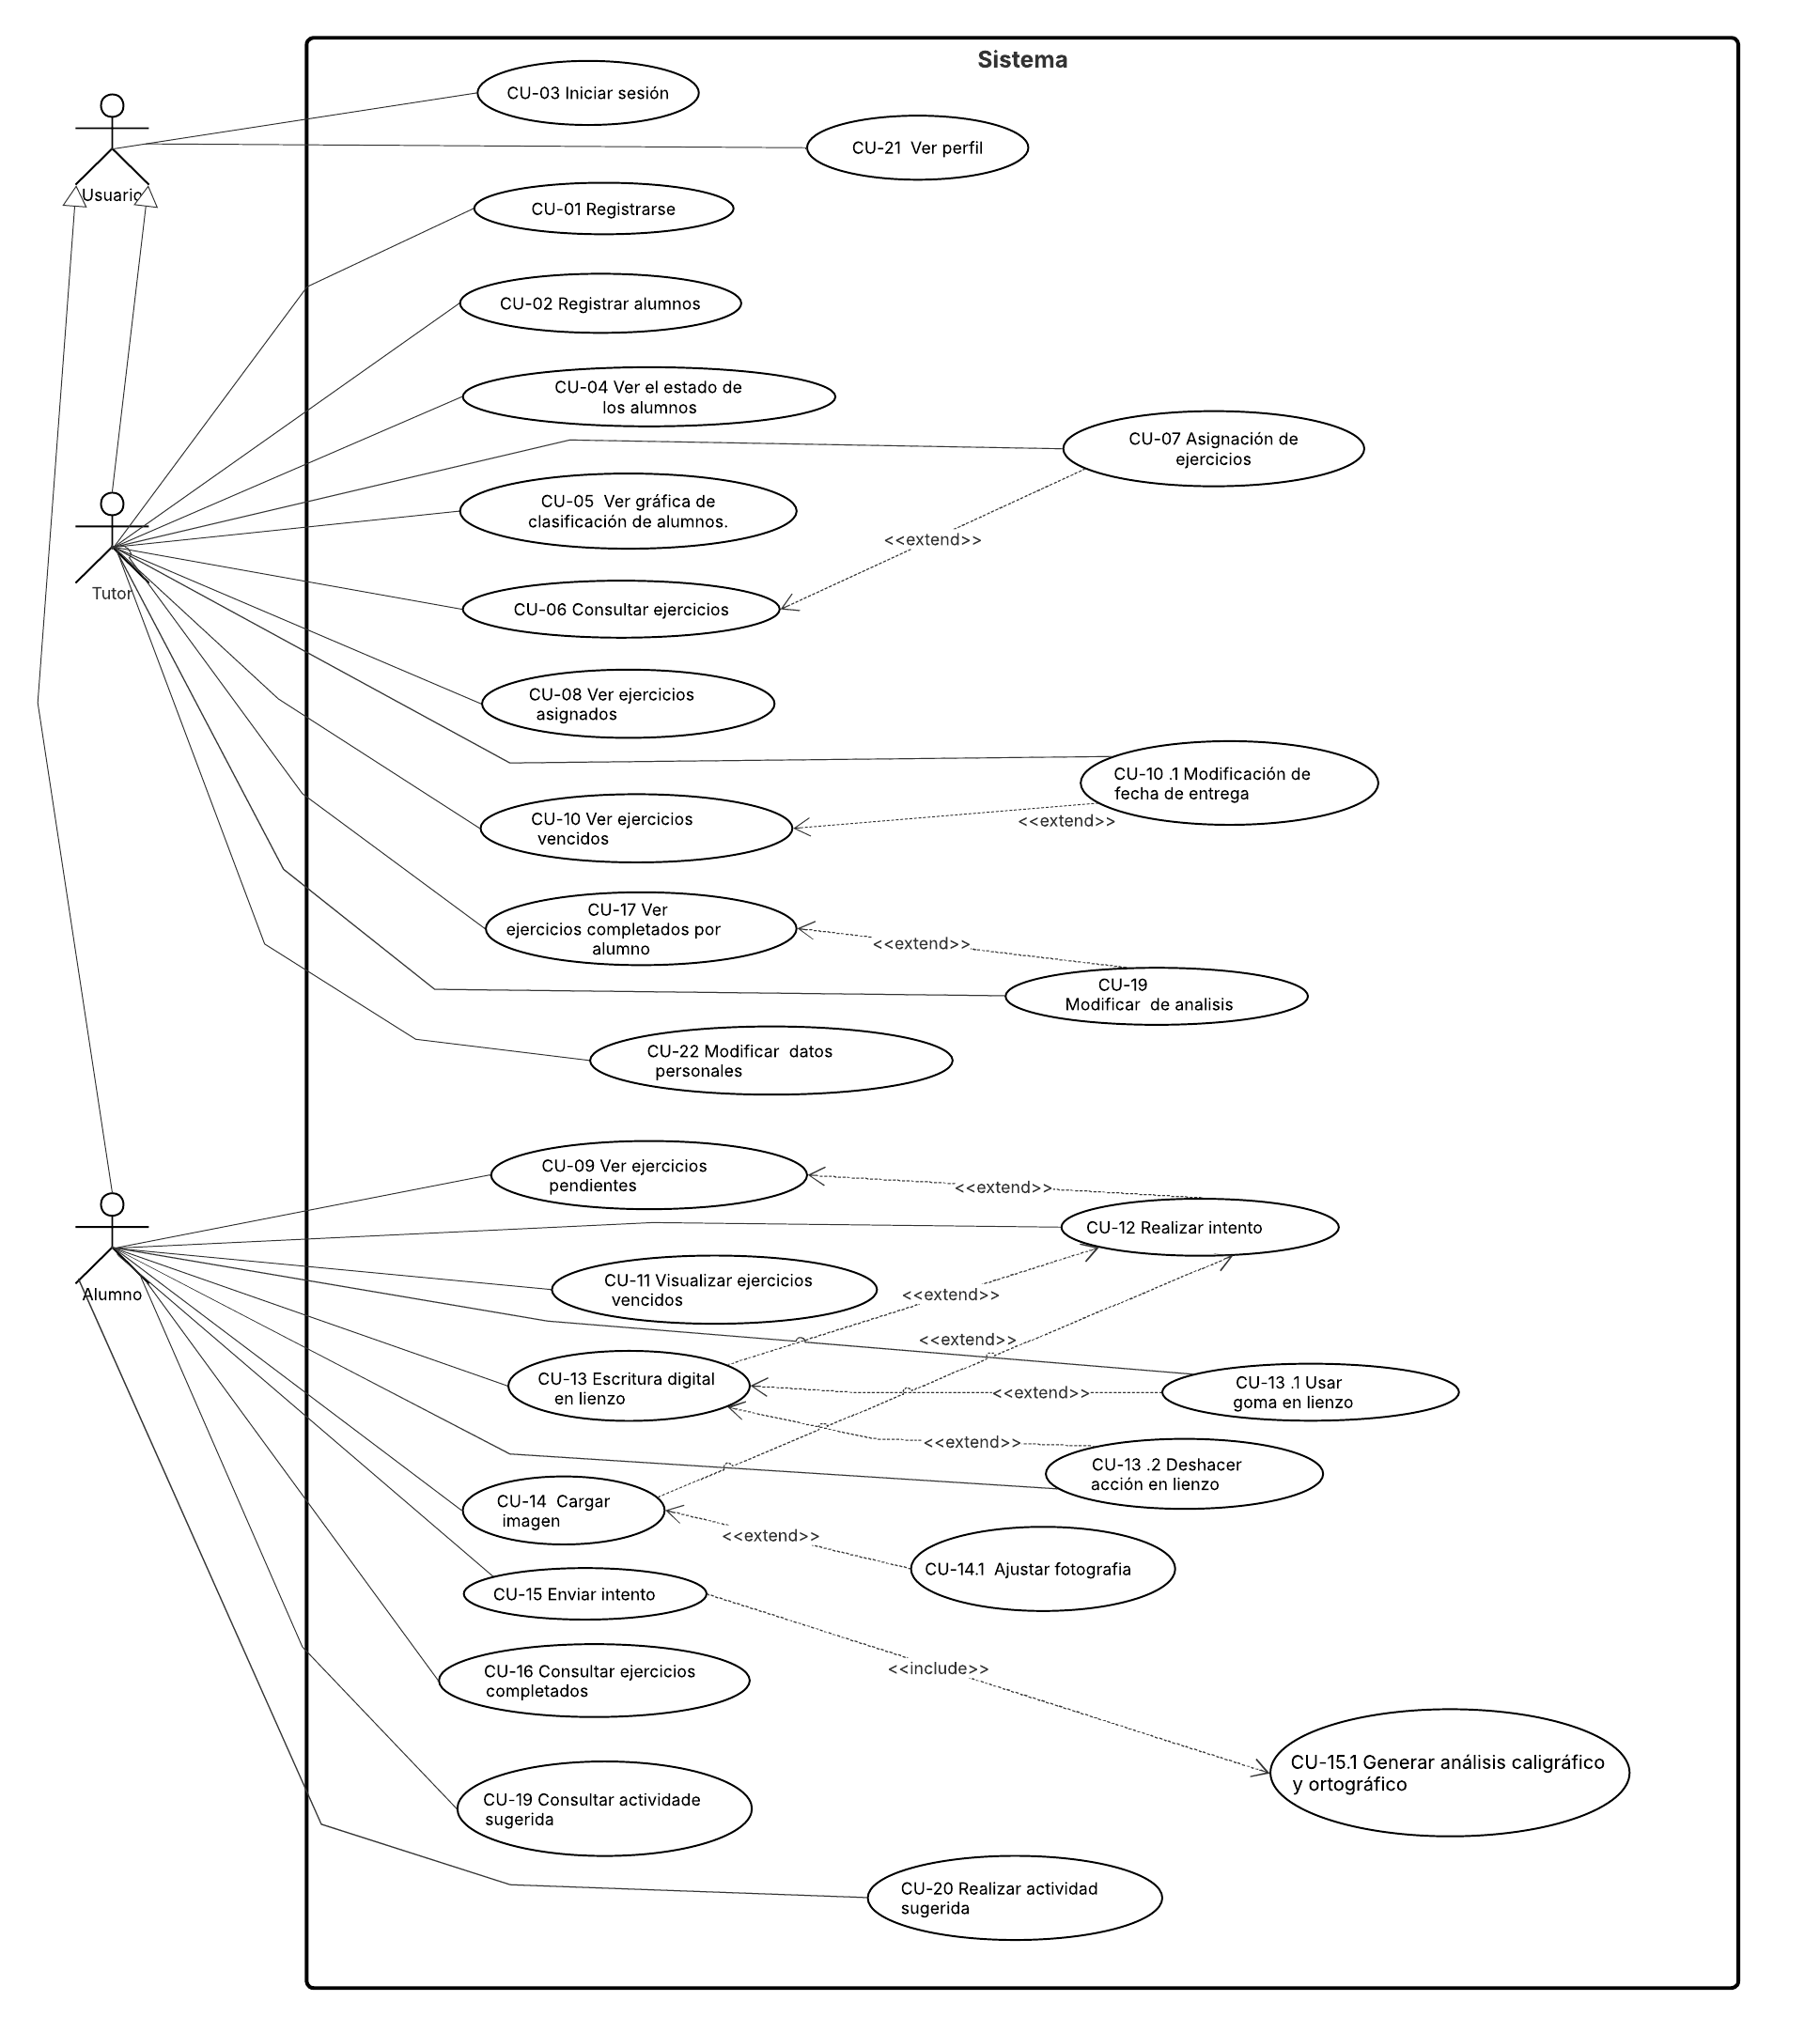
\includegraphics[height=0.82\textheight,keepaspectratio]{Imagenes/DiagramaCU-3.png}
  \caption{Diagrama de casos de uso}
\end{figure}

\subsubsection{Especificación de los casos de uso}

\begin{longtable}{|p{4cm}|p{11cm}|}
\caption{Tabla de especificación CU-01}
\label{tab:cu01} \\

\hline
\multicolumn{2}{|c|}{\textbf{CU-01 Registro de tutor}} \\
\hline
\endfirsthead

\hline
\multicolumn{2}{|c|}{\textbf{CU-01 Registro de tutor}} \\
\hline
\endhead

\hline
\endfoot

Actor & Tutor \\
\hline

Descripción & El tutor ingresa sus datos personales en el formulario de la aplicación web para crear su cuenta y acceder a sus funcionalidades. \\
\hline

Datos & Nombre, apellido paterno, nombre de usuario, correo electrónico, contraseña. \\
\hline

Estímulo & El tutor ingresa a la vista de registro, ingresa sus datos en el formulario y los envía. \\
\hline

Respuesta & La aplicación web valida los datos, crea la cuenta del tutor y le permite acceder a las funcionalidades del tutor. \\
\hline

Comentarios & El correo electrónico y nombre de usuario debe ser único en la aplicación web. \\
\hline

\end{longtable}

\begin{longtable}{|p{4cm}|p{11cm}|}
\caption{Tabla de especificación CU-02}
\label{tab:cu02} \\

\hline
\multicolumn{2}{|c|}{\textbf{CU-02 Registrar alumno}} \\
\hline
\endfirsthead

\hline
\multicolumn{2}{|c|}{\textbf{CU-02 Registrar alumno}} \\
\hline
\endhead

\hline
\endfoot

Actor & Tutor \\
\hline
Descripción & El tutor registra a un alumno en la aplicación web, ingresando sus datos e indicando el grado y grupo al que pertenece. \\
\hline
Datos & Nombre, apellido paterno, apellido materno, nombre de usuario, contraseña, grado y grupo. \\
\hline
Estímulo & El tutor, ya autenticado, ingresa a la vista ``Alumnos'', captura los datos en el formulario ``Alta de alumno'' y los envía. \\
\hline
Respuesta & La aplicación web registra los datos del alumno y lo asocia con el tutor responsable. \\
\hline
Comentarios & El nombre de usuario del alumno debe ser único. Solo tutores registrados pueden dar de alta alumnos. \\
\hline

\end{longtable}

%------------------------------------------------------

\begin{longtable}{|p{4cm}|p{11cm}|}
\caption{Tabla de especificación CU-03}
\label{tab:cu03} \\

\hline
\multicolumn{2}{|c|}{\textbf{CU-03 Iniciar sesión}} \\
\hline
\endfirsthead

\hline
\multicolumn{2}{|c|}{\textbf{CU-03 Iniciar sesión}} \\
\hline
\endhead

\hline
\endfoot

Actor & Tutor, Alumno \\
\hline
Descripción & El usuario ingresa sus credenciales para autenticarse y acceder a las funcionalidades según su rol. \\
\hline
Datos & Nombre de usuario y contraseña. \\
\hline
Estímulo & El usuario accede a la aplicación e ingresa sus credenciales en el formulario de inicio de sesión. \\
\hline
Respuesta & La aplicación valida las credenciales, identifica el rol y redirige a la vista correspondiente. \\
\hline
Comentarios & Si las credenciales son incorrectas, se muestra un mensaje de error. \\
\hline

\end{longtable}

%------------------------------------------------------

\begin{longtable}{|p{4cm}|p{11cm}|}
\caption{Tabla de especificación CU-04}
\label{tab:cu04} \\

\hline
\multicolumn{2}{|c|}{\textbf{CU-04 Ver el estado de los alumnos}} \\
\hline
\endfirsthead

\hline
\multicolumn{2}{|c|}{\textbf{CU-04 Ver el estado de los alumnos}} \\
\hline
\endhead

\hline
\endfoot

Actor & Tutor \\
\hline
Descripción & El tutor consulta el estado de desempeño de sus alumnos clasificados como bajo, regular y excelencia. \\
\hline
Datos & Lista de alumnos clasificados y métricas de progreso. \\
\hline
Estímulo & El tutor autenticado accede a su panel principal. \\
\hline
Respuesta & La aplicación muestra la lista de alumnos agrupados por categoría de desempeño. \\
\hline
Comentarios & Solo se muestran alumnos asociados al tutor autenticado. \\
\hline

\end{longtable}

%------------------------------------------------------

\begin{longtable}{|p{4cm}|p{11cm}|}
\caption{Tabla de especificación CU-05}
\label{tab:cu05} \\

\hline
\multicolumn{2}{|c|}{\textbf{CU-05 Ver gráfica de clasificación de alumnos}} \\
\hline
\endfirsthead

\hline
\multicolumn{2}{|c|}{\textbf{CU-05 er gráfica de clasificación de alumnos}} \\
\hline
\endhead

\hline
\endfoot

Actor & Tutor \\
\hline
Descripción & La aplicación presenta al tutor un gráfico con la distribución de alumnos según su nivel de desempeño. \\
\hline
Datos & Cantidad de alumnos en bajo, regular y excelencia. \\
\hline
Estímulo & El tutor accede al panel principal donde se muestra el gráfico. \\
\hline
Respuesta & La aplicación genera y actualiza dinámicamente el gráfico. \\
\hline
Comentarios & Puede mostrarse mediante gráfica de barras o anillo. \\
\hline

\end{longtable}

%------------------------------------------------------

\begin{longtable}{|p{4cm}|p{11cm}|}
\caption{Tabla de especificación CU-06}
\label{tab:cu06} \\

\hline
\multicolumn{2}{|c|}{\textbf{CU-06 Consultar ejercicios}} \\
\hline
\endfirsthead

\hline
\multicolumn{2}{|c|}{\textbf{CU-06 Consultar ejercicios}} \\
\hline
\endhead

\hline
\endfoot

Actor & Tutor \\
\hline
Descripción & La aplicación presenta al tutor el catálogo de ejercicios disponibles para asignar. \\
\hline
Datos & Nombre, descripción y contenido base del ejercicio. \\
\hline
Estímulo & El tutor accede a la sección de ejercicios. \\
\hline
Respuesta & La aplicación despliega el catálogo de ejercicios disponibles. \\
\hline
Comentarios & El tutor no crea ejercicios, solo los consulta y selecciona. \\
\hline

\end{longtable}

%------------------------------------------------------

\begin{longtable}{|p{4cm}|p{11cm}|}
\caption{Tabla de especificación CU-07}
\label{tab:cu07} \\

\hline
\multicolumn{2}{|c|}{\textbf{CU-07 Asignación de ejercicios}} \\
\hline
\endfirsthead

\hline
\multicolumn{2}{|c|}{\textbf{CU-07 Asignación de ejercicios}} \\
\hline
\endhead

\hline
\endfoot

Actor & Tutor \\
\hline
Descripción & El tutor selecciona uno o más ejercicios del catálogo y los activa para sus alumnos. \\
\hline
Datos & Ejercicios seleccionados, fecha límite opcional. \\
\hline
Estímulo & El tutor selecciona ejercicios y confirma la activación. \\
\hline
Respuesta & La aplicación registra los ejercicios activos y los publica a los alumnos. \\
\hline
Comentarios & La fecha límite es opcional. \\
\hline

\end{longtable}

%------------------------------------------------------

\begin{longtable}{|p{4cm}|p{11cm}|}
\caption{Tabla de especificación CU-08}
\label{tab:cu08} \\

\hline
\multicolumn{2}{|c|}{\textbf{CU-08 Ver ejercicios asignados}} \\
\hline
\endfirsthead

\hline
\multicolumn{2}{|c|}{\textbf{CU-08 Ver ejercicios asignados}} \\
\hline
\endhead

\hline
\endfoot

Actor & Tutor \\
\hline
Descripción & El tutor consulta la lista de ejercicios activados y sus fechas límite. \\
\hline
Datos & Ejercicios activos y fecha de entrega. \\
\hline
Estímulo & El tutor accede al módulo de ejercicios asignados. \\
\hline
Respuesta & La aplicación muestra los ejercicios seleccionados por el tutor. \\
\hline
Comentarios & Debe distinguir ejercicios con y sin fecha límite. \\
\hline

\end{longtable}

%------------------------------------------------------

\begin{longtable}{|p{4cm}|p{11cm}|}
\caption{Tabla de especificación CU-09}
\label{tab:cu09} \\

\hline
\multicolumn{2}{|c|}{\textbf{CU-09 Ver ejercicios pendientes}} \\
\hline
\endfirsthead

\hline
\multicolumn{2}{|c|}{\textbf{CU-09 Ver ejercicios pendientes}} \\
\hline
\endhead

\hline
\endfoot

Actor & Alumno \\
\hline
Descripción & El alumno consulta los ejercicios pendientes asignados por el tutor. \\
\hline
Datos & Nombre del ejercicio, descripción y fecha límite. \\
\hline
Estímulo & El alumno accede a la sección de ejercicios pendientes. \\
\hline
Respuesta & La aplicación muestra la lista de ejercicios activos no completados. \\
\hline
Comentarios & Solo se muestran ejercicios vigentes. \\
\hline

\end{longtable}

% CU-10
\begin{longtable}{|p{4cm}|p{11cm}|}
\caption{Tabla de especificación CU-10}
\label{tab:cu10} \\

\hline
\multicolumn{2}{|c|}{\textbf{CU-10 Visualización de ejercicios vencidos}} \\
\hline
\endfirsthead

\hline
\multicolumn{2}{|c|}{\textbf{CU-10 Visualización de ejercicios vencidos}} \\
\hline
\endhead

\hline
\endfoot

Actor & Tutor \\
\hline

Descripción & El tutor consulta la lista de ejercicios cuya fecha límite de entrega ha expirado, con el fin de decidir si extiende el plazo para uno o más de ellos. \\
\hline

Datos & Ejercicios seleccionados vencidos, fecha de entrega. \\
\hline

Estímulo & El tutor accede a la sección de ejercicios desde su panel de gestión y filtra los ejercicios seleccionados. \\
\hline

Respuesta & La aplicación web muestra únicamente los ejercicios activados por ese tutor, indicando para cada uno su fecha límite de entrega si fue establecida. \\
\hline

Comentarios & Debe distinguirse visualmente si un ejercicio fue seleccionado y ya está vencido. \\
\hline

\end{longtable}


% CU-11
\begin{longtable}{|p{4cm}|p{11cm}|}
\caption{Tabla de especificación CU-11}
\label{tab:cu11} \\

\hline
\multicolumn{2}{|c|}{\textbf{CU-11 Visualización de ejercicios vencidos}} \\
\hline
\endfirsthead

\hline
\multicolumn{2}{|c|}{\textbf{CU-11 Visualización de ejercicios vencidos}} \\
\hline
\endhead

\hline
\endfoot

Actor & Alumno \\
\hline

Descripción & El alumno consulta los ejercicios vencidos y no completados para conocer su estado y verificar si el tutor ha extendido el plazo de entrega. \\
\hline

Datos & Lista de ejercicios vencidos con nombre, fecha límite original y estado de habilitación por parte del tutor. \\
\hline

Estímulo & El alumno, autenticado en la aplicación web, accede a la sección de ejercicios vencidos desde su panel principal. \\
\hline

Respuesta & La aplicación web muestra los ejercicios no completados a tiempo, indicando si el tutor ha habilitado o no su entrega posterior. \\
\hline

Comentarios & Se debe distinguir entre ejercicios vencidos sin extensión y aquellos que el tutor habilitó nuevamente. \\
\hline

\end{longtable}


% CU-12
\begin{longtable}{|p{4cm}|p{11cm}|}
\caption{Tabla de especificación CU-12}
\label{tab:cu12} \\

\hline
\multicolumn{2}{|c|}{\textbf{CU-12 Realizar intento de ejercicio pendiente}} \\
\hline
\endfirsthead

\hline
\multicolumn{2}{|c|}{\textbf{CU-12 Realizar intento de ejercicio pendiente}} \\
\hline
\endhead

\hline
\endfoot

Actor & Alumno \\
\hline

Descripción & El alumno selecciona un ejercicio pendiente asignado por el tutor y accede a la vista de captura de escritura para realizarlo. \\
\hline

Datos & Datos del ejercicio seleccionado. \\
\hline

Estímulo & El alumno elige un ejercicio de su lista de pendientes y confirma que desea realizarlo. \\
\hline

Respuesta & La aplicación web carga la vista de captura de escritura correspondiente al ejercicio seleccionado, habilitando las herramientas para que el alumno lo complete. \\
\hline

Comentarios & Solo se pueden realizar ejercicios de plazo vigente o extensión habilitada. \\
\hline

\end{longtable}

% CU-13
\begin{longtable}{|p{4cm}|p{11cm}|}
\caption{Tabla de especificación CU-13}
\label{tab:cu13} \\

\hline
\multicolumn{2}{|c|}{\textbf{CU-13 Escritura digital en lienzo}} \\
\hline
\endfirsthead

\hline
\multicolumn{2}{|c|}{\textbf{CU-13 Escritura digital en lienzo}} \\
\hline
\endhead

\hline
\endfoot

Actor & Alumno \\
\hline

Descripción & El alumno realiza el ejercicio de escritura manuscrita directamente sobre un lienzo digital cuadriculado, utilizando herramientas de la aplicación web; como goma y deshacer para corregir su trazo. \\
\hline

Datos & Trazos digitales, acciones de corrección, datos del ejercicio seleccionado. \\
\hline

Estímulo & El alumno accede a la vista de captura (desde CU-12) y comienza a escribir sobre el lienzo digital con su dispositivo. \\
\hline

Respuesta & La aplicación web registra los trazos del alumno sobre el lienzo digital, habilitando las herramientas de corrección para que pueda corregir su trazo antes de enviarlo. \\
\hline

Comentarios & El lienzo debe ser compatible con entrada táctil o con lápiz digital según el dispositivo. Esta opción es alternativa a CU-14 (carga de fotografía); el alumno usa una u otra. \\
\hline

\end{longtable}


% CU-13.1
\begin{longtable}{|p{4cm}|p{11cm}|}
\caption{Tabla de especificación CU-13.1}
\label{tab:cu13-1} \\

\hline
\multicolumn{2}{|c|}{\textbf{CU-13.1 Uso de goma en lienzo}} \\
\hline
\endfirsthead

\hline
\multicolumn{2}{|c|}{\textbf{CU-13.1 Uso de goma en lienzo}} \\
\hline
\endhead

\hline
\endfoot

Actor & Alumno \\
\hline

Descripción & El alumno utiliza la herramienta de goma para corregir errores en su escritura sobre el lienzo digital antes de enviar el ejercicio. \\
\hline

Datos & Área o trazo seleccionado para borrar. \\
\hline

Estímulo & El alumno, dentro de la vista del lienzo (CU-13), identifica un error en una parte específica de su escritura, selecciona la herramienta de goma y arrastra sobre el trazo que desea eliminar. \\
\hline

Respuesta & La aplicación web elimina únicamente el área o trazo que el alumno cubrió con la goma. \\
\hline

Comentarios & La goma permite una corrección selectiva y precisa. \\
\hline

\end{longtable}

% =========================
% CU-13.2
% =========================
\begin{longtable}{|p{4cm}|p{11cm}|}
\caption{Tabla de especificación CU-13.2}
\label{tab:cu13-2} \\

\hline
\multicolumn{2}{|c|}{\textbf{CU-13.2 Deshacer acción en lienzo}} \\
\hline
\endfirsthead

\hline
\multicolumn{2}{|c|}{\textbf{CU-13.2 Deshacer acción en lienzo}} \\
\hline
\endhead

\hline
\endfoot

Actor & Alumno \\
\hline

Descripción & El alumno utiliza la acción de deshacer para revertir el último trazo completo registrado en el lienzo digital. \\
\hline

Datos & Historial de trazos registrados en el lienzo, último trazo a revertir, estado del lienzo tras la acción de deshacer. \\
\hline

Estímulo & El alumno, dentro de la vista del lienzo (CU-13), identifica que su última acción en el lienzo fue incorrecta y presiona el botón de “Deshacer”. \\
\hline

Respuesta & La aplicación web revierte la última acción realizada por el alumno. \\
\hline

Comentarios & Puede ejecutarse de forma consecutiva para revertir múltiples acciones. \\
\hline

\end{longtable}


% =========================
% CU-14
% =========================
\begin{longtable}{|p{4cm}|p{11cm}|}
\caption{Tabla de especificación CU-14}
\label{tab:cu14} \\

\hline
\multicolumn{2}{|c|}{\textbf{CU-14 Cargar imagen como alternativa}} \\
\hline
\endfirsthead

\hline
\multicolumn{2}{|c|}{\textbf{CU-14 Cargar imagen como alternativa}} \\
\hline
\endhead

\hline
\endfoot

Actor & Alumno \\
\hline

Descripción & El alumno sube una imagen como alternativa al lienzo digital, ya sea tomando una foto con la cámara del dispositivo o subiendo un archivo de imagen guardado. \\
\hline

Datos & Archivo de imagen (fotografía o imagen digital de la escritura manuscrita en formatos JPG, PNG o similar), ejercicio al que corresponde el intento. \\
\hline

Estímulo & El alumno accede a la vista de captura (desde CU-12), selecciona la opción de subir foto y elige “Tomar foto” o “Subir archivo”. \\
\hline

Respuesta & La aplicación web recibe la imagen cargada, muestra una vista previa para que el alumno la confirme y la asocia al intento del ejercicio, dejándola lista para su envío a revisión. \\
\hline

Comentarios & Es recomendable validar el tamaño y calidad mínima de la imagen. Esta opción es alternativa a CU-13; el alumno usa una u otra desde la misma vista de captura. \\
\hline

\end{longtable}


% =========================
% CU-14.1
% =========================
\begin{longtable}{|p{4cm}|p{11cm}|}
\caption{Tabla de especificación CU-14.1}
\label{tab:cu14-1} \\

\hline
\multicolumn{2}{|c|}{\textbf{CU-14.1 Ajustar fotografía}} \\
\hline
\endfirsthead

\hline
\multicolumn{2}{|c|}{\textbf{CU-14.1 Ajustar fotografía}} \\
\hline
\endhead

\hline
\endfoot

Actor & Alumno \\
\hline

Descripción & El alumno ajusta la fotografía antes de confirmarla. \\
\hline

Datos & Fotografía capturada en el momento, ajustes aplicados (recorte, rotación). \\
\hline

Estímulo & El alumno, tras tomar la foto con la cámara (CU-14), visualiza la vista previa y decide ajustarla antes de confirmarla. \\
\hline

Respuesta & La aplicación web aplica los ajustes y muestra la imagen corregida en la vista previa, lista para ser enviada a revisión. \\
\hline

Comentarios & Este caso solo aplica cuando el alumno eligió “Tomar foto”. \\
\hline

\end{longtable}


% =========================
% CU-15
% =========================
\begin{longtable}{|p{4cm}|p{11cm}|}
\caption{Tabla de especificación CU-15}
\label{tab:cu15} \\

\hline
\multicolumn{2}{|c|}{\textbf{CU-15 Enviar intento}} \\
\hline
\endfirsthead

\hline
\multicolumn{2}{|c|}{\textbf{CU-15 Enviar intento}} \\
\hline
\endhead

\hline
\endfoot

Actor & Alumno \\
\hline

Descripción & El alumno envía su ejercicio completado a la aplicación web para que sea analizado, una vez que considera que su escritura está lista, usando el botón de envío disponible en la misma vista de captura. \\
\hline

Datos & Intento del ejercicio (imagen cargada), ejercicio al que corresponde, alumno autenticado, fecha y hora de envío. \\
\hline

Estímulo & El alumno revisa su escritura en la vista de captura y presiona el botón “Enviar Revisión”. \\
\hline

Respuesta & La aplicación web registra el envío, marca el ejercicio como entregado, lo pone a disposición de los modelos de análisis y confirma al alumno que el envío fue exitoso. \\
\hline

Comentarios & Una vez enviado, el ejercicio no puede modificarse. Este es el último paso de CU-13 o CU-14. \\
\hline

\end{longtable}


% =========================
% CU-15.1
% =========================
\begin{longtable}{|p{4cm}|p{11cm}|}
\caption{Tabla de especificación CU-15.1}
\label{tab:cu15_1} \\
\hline
\multicolumn{2}{|c|}{\textbf{CU-15.1 Generar análisis caligráfico y ortográfico}} \\
\hline
\endfirsthead
\hline
\multicolumn{2}{|c|}{\textbf{CU-15.1 Generar análisis caligráfico y ortográfico}} \\
\hline
\endhead
\hline
\endfoot
Actor & Ninguno (proceso interno de la aplicación web) \\
\hline
Descripción & El sistema analiza automáticamente el intento de escritura enviado por el alumno, evaluando aspectos caligráficos y ortográficos mediante los módulos internos de OCR y NLP, con el fin de generar un resultado que refleje el desempeño del alumno. \\
\hline
Datos & Imagen del intento enviado (trazo digital o fotografía), identificador del ejercicio, identificador del alumno, resultado del análisis caligráfico y ortográfico generado por los módulos OCR y NLP. \\
\hline
Estímulo & El módulo de análisis se activa automáticamente una vez que el alumno confirma el envío del ejercicio en CU-15. \\
\hline
Respuesta & El módulo procesa la imagen mediante OCR para extraer el contenido escrito y aplica NLP para evaluar la ortografía y caligrafía. Los resultados del análisis se almacenan y quedan disponibles para el alumno en CU-16 y para el tutor en CU-17. \\
\hline
Comentarios & Este caso de uso es un \textit{\textlangle\textlangle include\textrangle\textrangle} de CU-15, ya que el análisis siempre ocurre tras cada envío sin excepción. Al tratarse de un proceso interno, no requiere intervención del usuario.  \\
\hline
\end{longtable}

% =========================
% CU-16
% =========================
\begin{longtable}{|p{4cm}|p{11cm}|}
\caption{Tabla de especificación CU-16}
\label{tab:cu16} \\

\hline
\multicolumn{2}{|c|}{\textbf{CU-16 Ver ejercicios completados}} \\
\hline
\endfirsthead

\hline
\multicolumn{2}{|c|}{\textbf{CU-16 Ver ejercicios completados}} \\
\hline
\endhead

\hline
\endfoot

Actor & Alumno \\
\hline

Descripción & El alumno consulta el historial de ejercicios que ha completado y enviado, junto con los resultados del análisis ortográfico y caligráfico obtenidos en cada uno. \\
\hline

Datos & Lista de ejercicios completados con nombre del ejercicio, fecha de entrega y resultados de escritura (análisis ortográfico y caligráfico). \\
\hline

Estímulo & El alumno autenticado, accede a la sección de ejercicios completados desde su panel principal. \\
\hline

Respuesta & La aplicación web muestra el historial de ejercicios completados por el alumno, mostrando para cada ejercicio el resultado de su análisis. \\
\hline

Comentarios & Solo se muestran ejercicios que el alumno haya enviado previamente (CU-15). Los resultados deben estar disponibles una vez que la aplicación web haya procesado el análisis del ejercicio enviado. \\
\hline

\end{longtable}

% =========================
% CU-17
% =========================
\begin{longtable}{|p{4cm}|p{11cm}|}
\caption{Tabla de especificación CU-17}
\label{tab:cu17} \\

\hline
\multicolumn{2}{|c|}{\textbf{CU-17 Ver ejercicios completados por alumno}} \\
\hline
\endfirsthead

\hline
\multicolumn{2}{|c|}{\textbf{CU-17 Ver ejercicios completados por alumno}} \\
\hline
\endhead

\hline
\endfoot

Actor & Tutor \\
\hline

Descripción & El tutor consulta las actividades realizadas por cada alumno, incluyendo los resultados del análisis ortográfico y caligráfico obtenidos en los ejercicios completados. \\
\hline

Datos & Lista de alumnos con sus ejercicios completados, fecha de entrega y resultados de escritura correspondientes a cada intento. \\
\hline

Estímulo & El tutor accede a la vista de alumnos y selecciona al alumno que desea consultar. \\
\hline

Respuesta & La aplicación web muestra el historial de ejercicios completados por el alumno seleccionado, incluyendo los resultados del análisis de escritura para cada uno. \\
\hline

Comentarios & Solo se muestran alumnos vinculados al tutor autenticado. Este caso de uso es el punto de entrada a CU-18, donde el tutor puede modificar los resultados si no está de acuerdo con el análisis. \\
\hline

\end{longtable}


% =========================
% CU-18
% =========================
\begin{longtable}{|p{4cm}|p{11cm}|}
\caption{Tabla de especificación CU-18}
\label{tab:cu18} \\

\hline
\multicolumn{2}{|c|}{\textbf{CU-18 Modificar análisis}} \\
\hline
\endfirsthead

\hline
\multicolumn{2}{|c|}{\textbf{CU-18 Modificar análisis}} \\
\hline
\endhead

\hline
\endfoot

Actor & Tutor \\
\hline

Descripción & El tutor modifica los resultados del análisis ortográfico y caligráfico de un ejercicio realizado por un alumno, en caso que el análisis de la aplicación web no refleja correctamente su desempeño. \\
\hline

Datos & Ejercicio seleccionado, resultados originales del análisis automático, correcciones o ajustes realizados por el tutor, alumno al que corresponde el intento. \\
\hline

Estímulo & El tutor accede a la vista de alumnos, selecciona al alumno que desea consultar, el ejercicio completado y elige la opción de modificar análisis. \\
\hline

Respuesta & La aplicación guarda los cambios realizados por el tutor, actualiza los resultados del ejercicio y los refleja en la vista del alumno (CU-16). \\
\hline

Comentarios & Solo el tutor responsable del alumno puede modificar sus resultados. \\
\hline

\end{longtable}


% =========================
% CU-19
% =========================
\begin{longtable}{|p{4cm}|p{11cm}|}
\caption{Tabla de especificación CU-19}
\label{tab:cu19} \\

\hline
\multicolumn{2}{|c|}{\textbf{CU-19 Consultar actividades sugeridas}} \\
\hline
\endfirsthead

\hline
\multicolumn{2}{|c|}{\textbf{CU-19 Consultar actividades sugeridas}} \\
\hline
\endhead

\hline
\endfoot

Actor & Alumno \\
\hline

Descripción & El alumno consulta las actividades de mejora sugeridas por la aplicación web, recomendadas a partir de los resultados de sus análisis ortográficos y caligráficos previos. \\
\hline

Datos & Lista de recomendaciones con actividades sugeridas (nombre de la actividad, descripción y área de mejora asociada ortografía o caligrafía), vinculados al intento realizado. \\
\hline

Estímulo & El alumno, accede a la sección de actividades sugeridas desde su panel principal. \\
\hline

Respuesta & La aplicación web muestra las actividades recomendadas personalizadas para el alumno, basadas en las áreas de oportunidad detectadas en sus análisis de escritura. \\
\hline

Comentarios & Si el alumno no tiene ejercicios completados aún, esta sección puede estar vacía o mostrar un mensaje orientador. \\
\hline

\end{longtable}


% =========================
% CU-20
% =========================
\begin{longtable}{|p{4cm}|p{11cm}|}
\caption{Tabla de especificación CU-20}
\label{tab:cu20} \\

\hline
\multicolumn{2}{|c|}{\textbf{CU-20 Realizar actividades sugeridas}} \\
\hline
\endfirsthead

\hline
\multicolumn{2}{|c|}{\textbf{CU-20 Realizar actividades sugeridas}} \\
\hline
\endhead

\hline
\endfoot

Actor & Alumno \\
\hline

Descripción & El alumno realiza una actividad sugerida por la aplicación web con el fin de trabajar en la mejora de los aspectos ortográficos y caligráficos identificados en sus análisis previos. \\
\hline

Datos & Actividad sugerida seleccionada, área de mejora asociada (ortografía o caligrafía). \\
\hline

Estímulo & El alumno, desde la sección de actividades sugeridas (CU-19), selecciona una actividad y confirma que desea realizarla. \\
\hline

Respuesta & La aplicación web carga la actividad seleccionada y registra el ejercicio realizado por el alumno. \\
\hline

Comentarios & Las actividades sugeridas son distintas a los ejercicios asignados por el tutor. \\
\hline

\end{longtable}

% =========================
% CU-21
% =========================
\begin{longtable}{|p{4cm}|p{11cm}|}
\caption{Tabla de especificación CU-21}
\label{tab:cu21} \\

\hline
\multicolumn{2}{|c|}{\textbf{CU-21 Ver perfil}} \\
\hline
\endfirsthead

\hline
\multicolumn{2}{|c|}{\textbf{CU-21 Ver perfil}} \\
\hline
\endhead

\hline
\endfoot

Actor & Tutor, Alumno \\
\hline

Descripción & El usuario podrá verificar sus datos personales en la vista de "Ver perfil". \\
\hline

Datos & Datos personales del usuario, registrados en la plataforma. \\
\hline

Estímulo & El usuario desde el panel principal accede a la vista de "Ver perfil". \\
\hline

Respuesta & La aplicación web carga la información del usuario. \\
\hline

Comentarios & Los alumnos no pueden modificar su información. \\
\hline

\end{longtable}

\begin{longtable}{|p{4cm}|p{11cm}|}
\caption{Tabla de especificación CU-22}
\label{tab:cu22} \\

\hline
\multicolumn{2}{|c|}{\textbf{CU-22 Modificar datos personales}} \\
\hline
\endfirsthead

\hline
\multicolumn{2}{|c|}{\textbf{CU-22 Modificar datos personales}} \\
\hline
\endhead

\hline
\endfoot

Actor & Tutor \\
\hline

Descripción & El podrá modificar sus datos personales, mostrados en la vista "Ver perfil". \\
\hline

Datos & Datos modificados por el tutor. \\
\hline

Estímulo & El tutor desde la vista "Ver perfil" preciona el botón para editar el campo que decida. \\
\hline

Respuesta & La aplicación web recibe el campo que se va a modificar y actualiza la pagina "Ver perfil" para visualizar sus datos modificados. \\
\hline

Comentarios & Solo el tutor puede modificar su información. \\
\hline

\end{longtable}

\subsection{Requerimientos del sistema.}

A continuación en esta sección se encuentran las Tablas \ref{tab:requerimientos_funcionales} y \ref{tab:rnf} donde se detallan los requerimientos funcionales del sistema y  los requerimientos no funcionales, así como sus tablas de especificación de requerimientos.